\documentclass[twocolumn]{article}

\usepackage{scrextend}
\changefontsizes{8pt}

\makeatletter
\renewcommand*{\fps@figure}{!htb}
\renewcommand*{\fps@table}{!htb}
\makeatother

\usepackage{sectsty}
\sectionfont{\fontsize{11}{11}\selectfont}
\subsectionfont{\fontsize{10}{11}\selectfont}

\usepackage[compact]{titlesec}
\titlespacing{\section}{0pt}{2ex}{1ex}
\titlespacing{\subsection}{0pt}{1ex}{1ex}
\titlespacing{\subsubsection}{0pt}{0.5ex}{1ex}

\setlength{\parskip}{0cm}
\setlength{\parindent}{1em}

\usepackage{geometry}
 \geometry{
 a4paper,
 total={170mm,257mm},
 left=20mm,
 top=20mm,
 }
\usepackage[utf8]{inputenc}
\usepackage[hidelinks]{hyperref}
\usepackage{amsmath, bm}
\usepackage[ruled,vlined]{algorithm2e}
\usepackage{amssymb}
\usepackage{graphicx}
\usepackage{float}
\usepackage{booktabs}
\usepackage[parfill]{parskip}
\usepackage{comment}
\usepackage{subcaption}
\usepackage{booktabs}



\usepackage{listings}
\lstset{
    language=Python,
    breaklines=true,
    breakatwhitespace=true,
    basicstyle=\footnotesize,
    frame=lines
}
\usepackage[capitalise, nameinlink]{cleveref}

\usepackage[sorting=none, style=verbose]{biblatex}
\addbibresource{lab_7.bib}

\usepackage{titling}
\setlength{\droptitle}{-1cm}

\title{\Large COMP6248 Lab 7 Exercise -- Transforming Sequences}
\author{\small Wei Chien Teoh (Eugene)\\\bigskip \href{mailto:wct1c16@soton.ac.uk}{wct1c16@soton.ac.uk}}
\date{\small 29 April 2021}

\begin{document}

\maketitle

\section*{Introduction}

The results are seeded using \lstinline{pytorch_lightning.seed_everything(0)} to provide reproducible results.

\section{Sequence-to-Sequence Modelling}

\subsection{Complete and train a sequence-to-sequence model}

\begin{lstlisting}[caption={Encoder class forward method.},language=Python]
    def forward(self, src):
        # TODO
        embedded = self.embedding(src)
        output, (hidden, cell) = self.rnn(embedded) # initial (hidden, cell) defaults to zero
        return hidden, cell
\end{lstlisting}

\begin{figure}
    \centering
    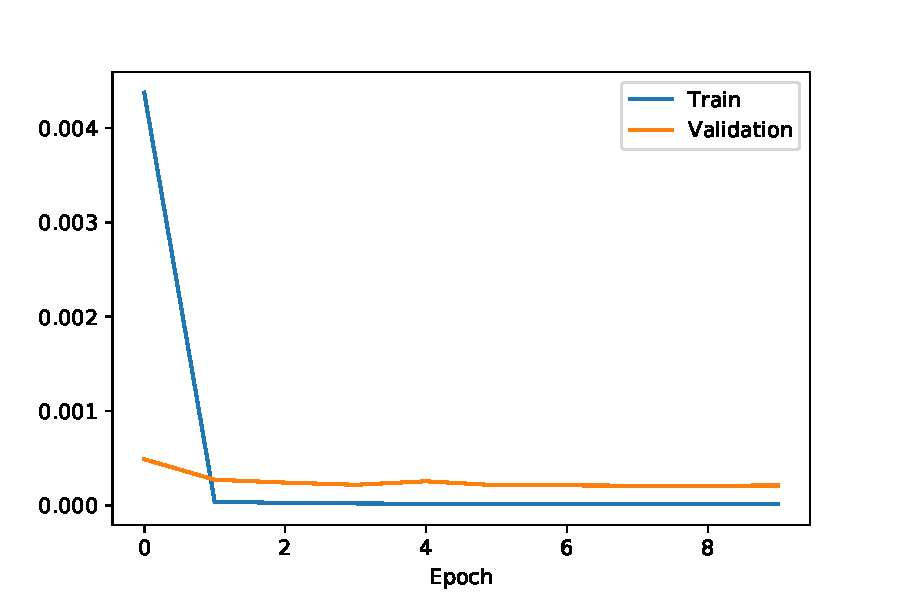
\includegraphics[width=\linewidth]{Figures/learning-curve.pdf}
    \caption{Loss curves for seq2seq model. Runtime: 9m 23s}
\end{figure}

\subsection{Now use it!}

\begin{lstlisting}[caption={Decoded output.},language={}]
    answer the following
    why is the order of the output reversed
    what is the point of teacher forcing
\end{lstlisting}


\subsubsection{Why is the order of the output reversed?}

In the seq2seq paper, it is discussed that reversing the source sentences results in better performance and memory utilization. This is possibly due to a ``stronger communication link'', where the first few words of the source sentences are closer to the first few words of the target sentences. The effects of reversing the output order achieves the same intuitive reasoning to reversing the source order. \cref{lst:reverse-output} shows a simple example for the intuition of this phenomenon \autocite{NlpWhyWe}.

\begin{lstlisting}[caption={Effects of reversed output order.},language={}, label={lst:reverse-output}]
    # original output order
    A B C -> alpha beta gamma

    # reversed output order
    # stronger link between (C, gamma), (B, beta)
    A B C -> gamma beta alpha
\end{lstlisting}

\subsubsection{What is the point of teacher forcing?}

Teacher forcing~\autocite{williamsLearningAlgorithmContinually1989} is a training strategy for RNN that uses ground truth as an input for the next time step. In sequence modelling, traditional MLL training that uses predicted output as input to the next sequence might provide large loss, which might result in slow convergence or stuck in bad local minima. Teacher forcing allows faster training. However, an extensive amount of teacher forcing might cause small prediction compound in the conditioning context \autocite{lambProfessorForcingNew2016}. Hence, in this model, a ratio (defaulting to 50\%) is introduced to control the percentage of which teacher forcing occurs.

\subsection{Sequence Lengths}

The original \lstinline{decode} function is modified to work with three set of code in one chunk, shown in \cref{lst:decode-long}. \cref{lst:output} shows the output of the function. The output shows missing letters in the start and end of the sentence. This suggests that the model failed to capture and predict long-term structure.

Although LSTMs are developed to better capture long-term structure, it still fails to perfectly achieve it.

The maximum sequence length in the training data is only 6. The short training sequence length is another issue of why the model does not have good performance on larger chunks.

\begin{lstlisting}[caption={Modified decode function with longer chunks.}, label={lst:decode-long}]
    def decode_long(code):
        out = ''

        # 3 spaces per element
        parts = code.split(' ')
        parts = [parts[i] + ' ' + parts[i+1] + ' ' + parts[i+2] for i in range(len(parts)-3)]

        for chunk in parts:
            num = ds.encode_morse('^ ' + chunk + ' $').unsqueeze(1)
            pred = model(num.cuda(), maxlen=2)
            pred = pred[1:].view(-1, pred_dim).argmax(-1)
            out += ds.decode_alpha(pred.cpu())[::-1]
        return out
\end{lstlisting}

\begin{lstlisting}[caption={Output of \lstinline{decode_long}.},language={}, label={lst:output}]
    code:
        .- -. ... .-- . .-. / - .... . / ..-. --- .-.. .-.. --- .-- .. -. --.
    decode:
        answer the following
    decode_long:
        swer the followin
\end{lstlisting}

\end{document}